%! TEX root=figure.1.tex

\documentclass{standalone}
\usepackage{physics}

\usepackage{kpfonts}

\usepackage{tikz}
\usetikzlibrary{arrows,calc,patterns}
\usetikzlibrary{positioning}


\usepackage{pgfplots}
\pgfplotsset{compat = 1.3}
\pgfplotsset{/pgfplots/error bars/error bar style={very thick}}

\begin{document}
    
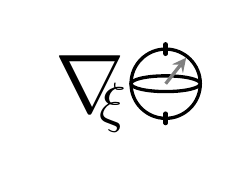
\begin{tikzpicture}[scale = .2]
        \coordinate (qubit) at (11, 4);
        \draw[very thick, black] (qubit) circle (2.2cm);
        \draw[very thick, black] (qubit) ellipse (2.2cm and 0.5cm);
        \draw[-stealth, very thick, color=gray] (qubit) to (12.3, 5.65);
        \draw[ultra thick,cap=round] (11,5.9) to (11,6.5);
        \draw[ultra thick,cap=round] (11,1.5) to (11,2.1);

        \node [left = .15 of qubit, scale=3] (nabla) {$\nabla$};
        \node [scale=2] at (7.65,2.5) {$\xi$};
        %\node[above] at (11.3,6.4) {\small{$\ket{0}_L$}};
        %\node[below] at (11.3,1.6) {\footnotesize{$\ket{1}_L$}};
\end{tikzpicture}

\end{document}
